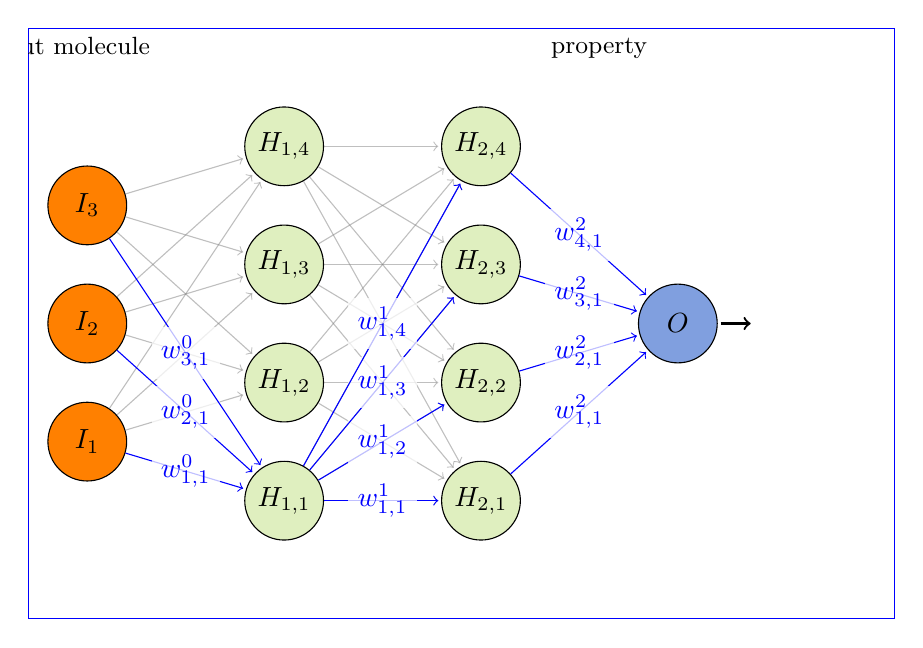
\begin{tikzpicture}[shorten >=1pt,draw=black, x=1cm, y=1 cm,  node distance=0cm]

\draw[use as bounding box, anchor = north west,draw=blue] (-2,-4.25) rectangle (9,3.25);
\clip (-2,-3.25) rectangle (9.0,3.25);

%% setup parameters for NN drawing

\tikzstyle{every pin edge}=[<-,shorten <=1pt,thick]
\tikzstyle{neuron}=[circle,fill=black!25,minimum size=1.0cm ,inner sep=0pt, color=black, draw]
\tikzstyle{input neuron}=[neuron, fill=green!25!blue!25];
\tikzstyle{output neuron}=[neuron, fill=green!25!blue!50];
\tikzstyle{hidden neuron}=[neuron, fill=green!50!orange!25];
\tikzstyle{annot} = [text width=2cm, text centered]


%% define coordinate grid 
\def \xfarleft {-1.25}
\def \xleft {-1.0}
\def \xmid {-0.25}
\def \xright {0.5}
\def \ytop {1.0}
\def \ymid {-0.5}
\def \ybot {-1.15}
\def \yphasetwo {-2.0}
\def \xlabeloffset {0.05}
\def \ylabeloffset {0.15}
\def\layersep{2.5}
\def\vlayersep{1.5}


% Draw the input layer nodes
\foreach \name/\y in {1/\ymid-\vlayersep,2/\ymid,3/\ymid+\vlayersep}{
\node[input neuron,fill=orange!100 ] (I-\name) at (\xfarleft,\y) {$I_{\name}$};}

% Draw the hidden layer nodes
\foreach \name/\y in {1/\ymid-1.5*\vlayersep,
2/\ymid-0.5*\vlayersep,
3/\ymid+0.5*\vlayersep,
4/\ymid+1.5*\vlayersep}{
{\path node[hidden neuron] (H-\name) at (\xfarleft+\layersep,\y) {$H_{1,\name}$};}
{\path node[hidden neuron] (H2-\name) at (\xfarleft+2*\layersep,\y) {$H_{2,\name}$};}
}


% Draw the output layer node
\node[thin, output neuron,pin={[pin edge={->}]right:\footnotesize }] at (\xfarleft+3*\layersep,\ymid) (O) {$O$};


%% hidden node connections 
\foreach \dest in {1,2,3,4}     
\foreach \source in {1,2,3,4}
{
{\path[thin,->,gray,opacity=0.5] (H-\source) edge node[font=\scriptsize] {$ $} (H2-\dest) ;}
}

\foreach \dest in {1,2,3,4}     
\foreach \source in {1}
{
{\path[thin,->,blue] (H-\source) edge node[rectangle, fill=white,fill opacity=0.75,text opacity=1] {\color{blue}$w_{\source,\dest}^{1}$} (H2-\dest) ;}
}


\foreach \source in {1,2,3,4}{
{\path[thin,->,blue] (H2-\source) edge node[rectangle, fill=white,fill opacity=0.75,text opacity=1] {\color{blue}$w_{\source,1}^{2}$} (O) ;}}



\foreach \source in {1,2,3}{
\foreach \dest in {2,3,4}{     
	\path[thin,->,gray,opacity=0.5] (I-\source) edge node[] {} (H-\dest) ;}}


\foreach \source in {1,2,3}{
\foreach \dest in {1}{     
	\path[thin,->,blue] (I-\source) edge node[rectangle, fill=white,fill opacity=0.75,text opacity=1] {\color{blue}$w_{\source,\dest}^{0}$} (H-\dest) ;}}




%\foreach \source in {2,3,4}{
%\foreach \dest in {1,2,3,4}{     
%	{\path[thin,->,opacity=0.5] (I-\source) edge node[font=\scriptsize] {} (H-\dest) ;}}
{\node [rotate=0] (ll) at (-1.5,3) {\small input molecule};}
{\node [rotate=0] (l2) at (5.25,3) {\small property};}


\end{tikzpicture}

